Después de varias pruebas descubrimos que el comportamiento de \texttt{SchedMistery} tiene el compartamiento de un \emph{multilevel feedback-queue}. Los parametros pasados son los quantums de las colas en orden de mayor a menos prioridad y tiene por defecto una cola de quantum 1 que es la de mayor prioridad.
\newline Detallamos los atributos privados y las funciones publicas de la clase \texttt{SchedNoMistery} donde replicamos el comportamiento de \texttt{SchedMistery}
Atributos privados:
\begin{itemize}
	\item \texttt{vq}: Es un vector que tiene las colas de prioridad en orden, la de mayor prioridad en el 0 y la de menor al final.
	\item \texttt{def\_quantum}: Tiene el quantum de cada una de las colas en vq. La cola en el subíndice i de vq tiene su respectivo quantum en el subíndice i de def\_quantum. 
	\item \texttt{unblock\_to}: Un vector hay un subíndice para cada proceso que tenga el procesador. Cuando un proceso se bloquea guarda en el subíndice pid la prioridad que le toca al desbloquearse. Esto funciona ya que los id de procesos empiezan en 0 y aumentan de a uno a medida que llegan.
	\item \texttt{quantum}: El quantum que le queda a el proceso que esta corriendo.
	\item \texttt{n}: La  cantidad de colas que tiene el scheduler.
	\item \texttt{cur\_pri}: La prioridad de la proceso que se esta corriendo
\end{itemize}

La clase tiene una función privada, \texttt{int next()}, que se encarga de devolver el \emph{pid} del siguiente proceso a ejecutar, buscado, desde la cola de mayor prioridad hasta la de menor, la primera cola vacia donde remueve el primer procesos, reinicia el \emph{quantum} y actualiza \emph{cur\_pri}. En caso de que todas las colas esten vacias devuelve el \emph{pid} de la tarea \emph{idle}.

Además posee los siguientes métodos públicos:
\begin{itemize}
	\item \texttt{SchedNoMistery(vector<int> argn)}: El constructor lee los quantum de las colas pasados como parámetros y los coloca en orden en def\_quantum y genera una cola vacia  para cada cola en vq, para así poder acceder más tarde. Además inicializa cur\_pri con 0, quantum como 1 y n como la cantidad de colas.
	\item \texttt{void load(int pid)}: Carga el proceso identificado por \texttt{pid} en la cola de mayor prioridad. 
	\item \texttt{void unblock(int pid)}: Agrega el proceso con id \texttt{pid} en la cola de prioridad indicada por el contenido del subíndice pid de \texttt{unblock\_to}.
	\item \texttt{int tick(int cpu, const enum Motivo m)}: Tiene tres casos según el motivo con el que se la haya llamado:
	\begin{enumerate}
		\item \texttt{Caso EXIT}: Simplemente llamamos a \texttt{next()} para que corra el siguiente proceso.
		\item \texttt{Caso BLOCK}: Guardo en \texttt{unblock\_to} en la posición del id del proceso que se corre, la prioridad actual menos uno. Después se llama a \texttt{next()} para que pueda correr el siguiete proceso.
		\item \texttt{TICK}: Pueden pasar varias cosas:
		\begin{enumerate}
			\item La tarea actual es \emph{idle}, en cuyo caso solo queda llamar a \texttt{next} y devolver su resultado.
			\item La tarea actual no es \emph{idle} pero se acabó su \emph{quantum}, por lo que hay que encolarla en la siguiente cola con menor prioridad y llamamos a \texttt{next}.
			\item La tarea actual ni es \emph{idle} ni terminó su \emph{quantum}, así que debe seguir ejecutando pero reducimos en 1 la cantidad de ciclos restantes.
		\end{enumerate}
	\end{enumerate}
\end{itemize}

Los diagramas \ref{fig:ej7-1} \ref{fig:ej7-2} \ref{fig:ej7-3} son los que más nos ayudaron para darnos cuenta como funcinaba \texttt{SchedMistery}.

\begin{figure}[H]
  \centering
  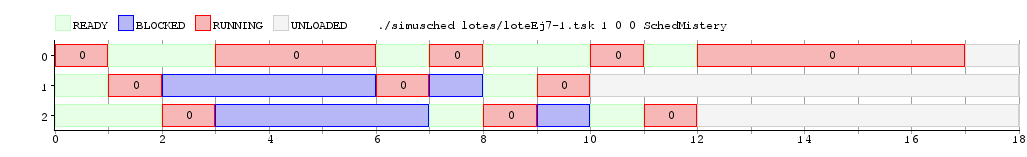
\includegraphics[width=1\textwidth]{img/imgEj7-1}
  \caption{}
  \label{fig:ej7-1}
\end{figure}

Para este diagrama no pasamos ningún parametro a \texttt{SchedMistery} lo que nos mostro que siempre tiene una cola de 1 de quantum. 

\begin{figure}[H]
  \centering
  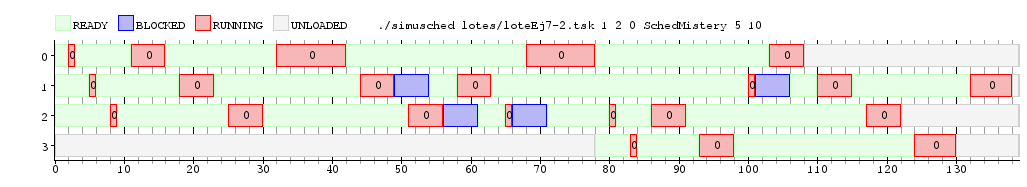
\includegraphics[width=1\textwidth]{img/imgEj7-2}
  \caption{}
  \label{fig:ej7-2}
\end{figure}

En este diagrama los quantums de las colas son 1, 5 y 10. Podemos observar que los tres procesos empiezan ejecutando quantum 1, después pasan a la segunda cola y ejecutan por 5 ciclos pasando a la tercera cola donde el proceso 0 gasta todo su quantum pero los procesos 1 y 2 se bloquean. Estos procesos pasan a la segunda cola, aumentando su prioridad, por eso el proceso 1 corre 5 ciclos, en cambio el proceso 2  se vuelve a bloquear y pasa a la primera cola. Como el proceso 1 entro último a la cola de menor prioridad y el proceso 2 esta bloqueado ejecuta el proceso 0. En el tiempo 78 entra el proceso 3 y se ubica al final de la primera cola, por esto se ejecuta el 2 (que había subido dos grados su prioridad) y luego el 3. Con esto pudimos ver que al gastar todo su quantum pasa a la siguiente cola con menor prioridad y al bloquearse  pasa a la siguiente cola con mayor prioridad.

\begin{figure}[H]
  \centering
  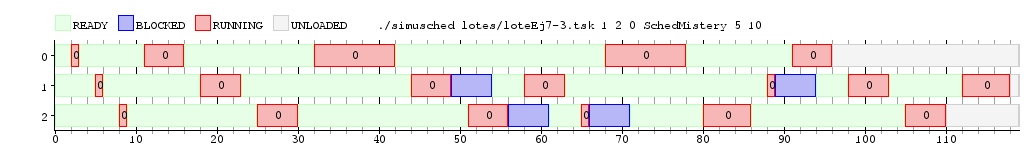
\includegraphics[width=1\textwidth]{img/imgEj7-3}
  \caption{}
  \label{fig:ej7-3}
\end{figure}

El lote usado para este diagrama es muy similar al anterior, la única diferencia es que no se agrega el proceso 3 en el tiempo 78. Esto genera que el proceso 2 cuando empieza a ejecutarse en el tiempo 80 ejecuta su quantum de 1 y como después de esto sigue siendo el más prioritario vuelve a ejecutar con el quantum de la segunda cola de prioridad (5), por eso ejecuta un total de 6 ciclos. Este gráfico nos mostro que para buscar al próximo proceso para ejecutarse siempre empezaba buscando en la cola de mayor prioridad hasta encontrar una cola que no estuviera vacia. Por lo que no ejecuta los de menor prioridad hasta acabar con los de mayor prioridad.